% !TEX root = ../main.tex


\chapter{Recursion proofs}

This chapter serves as an intermediary background exploration,
diving into more advanced concepts beyond last chapter concepts.
The realm of zero knowledge is dynamic and continuously evolving,
marked by ongoing advancements and active research endeavors. Among these advancements,
recursion proofs is one of the most important and active subjects. Recursion proofs are created to accelerate
the generation of multiple zero-knowledge proofs.
Recursion proofs differ in their design, they can vary significantly and serve different use cases.
In this section, we will examine these variations, distinguishing between them.
We aim to identify the most suitable method for our daily proof of liabilities and proof of inclusion. \cite{Nova23}



The prover's process in SNARKs is to create a proof using the setup parameters, a private witness, and public input. 
As discussed in the previous section, the proof begins by transforming the code into an arithmetic circuit, 
which is then represented as a polynomial. This polynomial is created using the witness (private input).

The objective is to demonstrate that the polynomial satisfies the solution without revealing the polynomial itself. 
This is where the \hyperref[subsec]{polynomial commitment scheme} becomes essential. 
The setup phase generates public parameters that assist in creating and verifying the proof without disclosing the polynomial.

\begin{figure}[H]
\centering
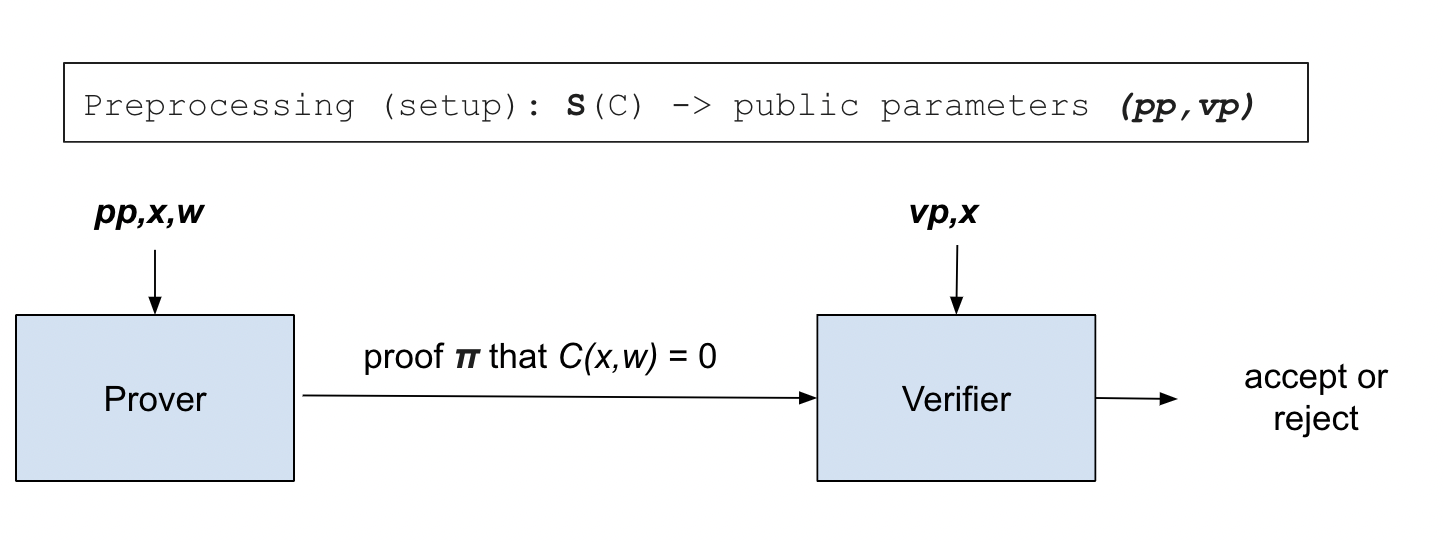
\includegraphics[width=130mm]{SNARKCircuit.png}
\caption{SNARK Circuit \cite{ZKM2}}
\label{overflow}
\end{figure}


\begin{itemize}
\item \textbf{S(C)}: Public parameters (pp,vp) for prover and verifier
\item \textbf{P(pp,x,w)}: Proof $\pi$
\item \textbf{V(vp,x,$\pi$)}: Accept or reject
\item \textbf{C(x,w)}: Arithmetic circuit
\item \textbf{w}: Private witness
\item \textbf{x}: Public input
\end{itemize}



\section{Aggregation}
 %-- Can expend on this using \cite{VRS23}, talk about proof composition
 Aggregation is the simplest form of recursion for zk proofs. Its purpose is to reduce the number of proofs that need to be verified. The process involves two phases.

 In the first phase, you create individual proofs for multiple blocks. In the second phase, these proofs are combined into a single "proof of proof". It takes multiple proof as input,
 and outputs a new proof validating the input proofs.
 This can be done either by merging all proofs into one or by creating a tree-like structure where each parent node verifies its child nodes.

This is a simple process. Each block has its own proof, and then you prove that the other proofs are valid, giving you only one prove
to verify at the end. Since there are 2 different phases, 2 different circuits need to be constructed.
On the surface, you can parallelize the initial proofs, which decrease the proving time, and you only have one proof to verify, which decreases the verifying time.
However, there are still some issues with aggregation. The most important issue is that the proof time of the second circuit grows linearly with the number of blocks to verify, making it less scalable. \cite{Nova23}
\iffalse
\begin{figure}[H]
   \centering
   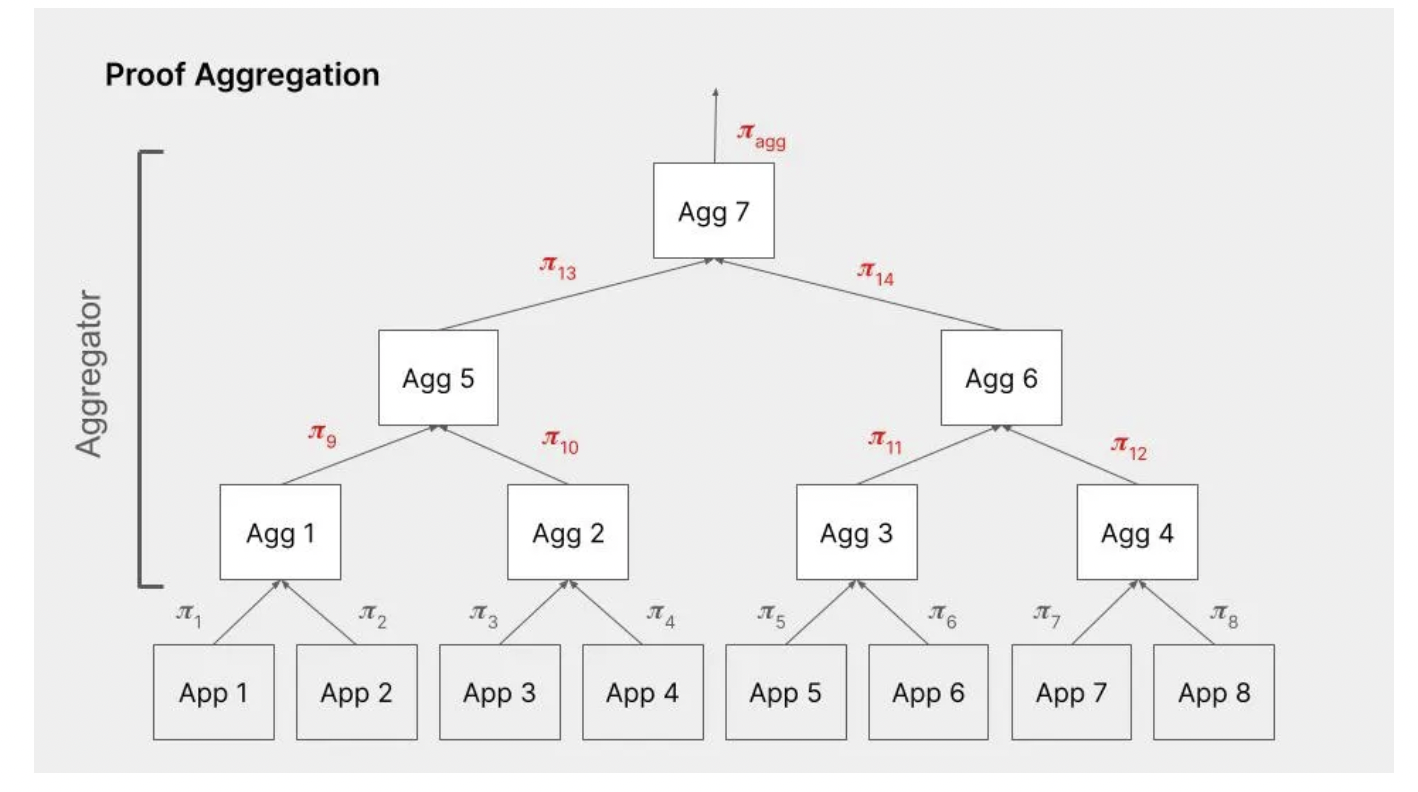
\includegraphics[width=130mm]{AggregationProof.png}
   \caption{Aggregation Proof \cite{TP24}}
   \label{overflow}
   \end{figure}
\fi

\section{Recursion scheme}
The next technique is the recursion scheme, or Incrementally Verifiable Computation (IVC). Like the aggregation, the proof is separated into blocks.
However, in this case each block serves two purposes. Provings that the block itself is valid, and that the previous proof is valid.
The number of constraints will always stay the same because it is only proving 2 things of fixed sizes. This creates
a chain structure, where verifying the latest block is the equivalent of verifying every block in the chain.
It is an improvement from the previous technique, because this allows to maintain a constant number of constraints in the circuit.
This implies that the latest does not take longer to verify than the second block.
However, each block still has to verify the previous block, which takes additional time. \cite{Nova23}
%-- Can Expend on this using \cite{VRS23}, talk about IVC


\section{Accumulation}
To mitigate the exponential growth of recursion proofs, the new scheme created by Nova defer every computationally heavy task to the end.
All the different parts are accumulated at a later point. Unlike the aggregation scheme, the last part of accumulation does not grow with every new step.
Instead of doing n times heavy work, we are doing it only once.
The heavy part of the verification step in most SNARKS is found when opening the polynomial commitment.


\subsection{Polynomial Commitments}
\label{subsec:pc}
A polynomial commitment is a cryptographic technique that allows to commit to (or "lock") a polynomial's data 
in such a way that the data can later be revealed (or "unlocked") while ensuring integrity and privacy.

Polynomial commitments are binding, meaning that once a commitment is made, it is impossible to alter the original polynomial without detection. 
The commitments are also much shorter than the polynomial data itself. While collisions are theoretically possible due to the pigeonhole principle, 
it is computationally infeasible to find a second polynomial that matches the same commitment.

Additionally, polynomial commitments can be hiding, which means no information about the polynomial is leaked to the verifier.
For example, we can create a commitment by hashing a polynomial with a collision-resistant hash function like SHA-256, and only the hash value is shared. 
To make it hiding, a random factor could be added to the polynomial data before hashing.

Instead of committing to a full dataset, we can commit specifically to a polynomial. 
Committing to the coefficients of the polynomial directly would reveal the polynomial when the commitment is opened. 
Instead, we want the ability to open the commitment only at a specific point of the polynomial, without revealing the entire polynomial itself. 
A polynomial commitment allows one party to prove to another that they possess a polynomial that evaluates to a certain value at a specific point without revealing any other information about the polynomial.
\cite{VR23}

There are many different polynomial schemes, such as KZG, Bulletproofs and FRI. 
In these schemes, the setup processes and the commitments vary significantly. 
KZG commitments rely on a trusted setup to generate elliptic curve parameters\cite{KZG}, Bulletproofs avoids the use of setup by using logarithm-based techniques\cite{BP18}, 
and FRI evaluates polynomial through proximity checks\cite{FRI} .
%-- few lines describing different polynomial schemes

\subsection{Halo accumulation}

The concept of deferring the polynomial commitment opening, and consolidating them into a single operation, was introduced by Bowe, Grigg, and Hopwood Halo.\cite{BGH23}
This process involves two parts:
the first part is fast, where you output a polynomial and its commitment.
The second part is expensive, where we verify the pair $(f_1, c_1)$ of the polynomial $f_1$ and its commitment $c_1$.
The second part can be accumulated if the commitment scheme is additively homomorphic.
Instead of individually verifying each pair, we accumulate the pairs and verify their linear combinations ($c_1+c_2+...$ is a commitment for $f_1+f_2+...$). \cite{VR23}

\section{Folding scheme}
Nova is an advanced polynomial commitment scheme designed to enhance the efficiency of recursive proofs by leveraging sophisticated accumulation techniques.
Instead of accumulating the hard part at the end, the folding scheme accumulates everything up until the end.
The setup is similar to the recursion scheme, but instead of computing the proof of the previous block, the R1CS are folded together at every block.
Instead of having $n$ set of R1CS, we are left with a single set. The new R1CS are called relaxed R1CS, and are used to compute a single proof at the end of the folding.
\cite{Nova23}  \cite{ASI23}


\subsection{Relaxed R1CS}
Going back to the previous \hyperref[subsec:r1cs]{section}, we previously defined what an R1CS is.
The goal is to combine 2 R1CS and obtain another R1CS. If we are able to do that, we can fold every R1CS together and be left with only one.
\\

If we \textbf{define our R1CS}:
\begin{quote}
\textbf{fix an R1CS} program $A,B,D \in \mathbb{F}^{u \times v}_p $
\\
We define $x$ as the public input, and $w$ as the witness.
\\
Instance 1: $ x_1 \in \mathbb{F}^n_p $, $ z_1 = (x_1, w_1) \in \mathbb{F}^v_p$
\\
Instance 2: $x_2 \in \mathbb{F}^n_p $, $ z_2 = (x_2, w_2) \in \mathbb{F}^v_p$
\\
Where $u$ is the number of constraints in the R1CS, $v$ is the number of variables in the constraint system, $p$ as the private field, and $n$ the number of public variables.
\\
We know $Az_i \circ Bz_i = Dz_i$ for $ i = 1,2$
\end{quote}


\textbf{Recall}: Our R1CS needs to be valid for any element of the field.
To prove this, the verifier choose a random point $r$ at which we will evaluate our constraints system.

\textbf{First attempt}:
\begin{quote}
Lets define $r$ as a random variable:
\\
$r \leftarrow \mathbb{F}_p$
\\
Then we set 
\\
$x \leftarrow x_1+rx_2$
\\
$z \leftarrow z_1 + rz_2 = (x_1+rx_2, w_1 + rw_2)$
\end{quote}


Then:
\begin{quote}
   $Az \circ Bz = A(z_1 + r z_2) \circ B(z_1 + rz_2)$
   \\
   $= (Az_1) \circ (Bz_1) + r^2 (Az_2) \circ (Bz_2) + (r(Az_2) \circ (Bz_1) + r(Az_1) \circ (Bz_2))$
   \\
   $=Dz_1 + r^2Dz_2 + E$
   \\
   Where $E$ is a combination of the remaining values.
   \\
\end{quote}
This is not quite an R1CS, because it is not of the form $Az_i \circ Bz_i = Dz_i$.
We need to modify the R1CS so that it can be folded.
\\
\\
Let's \textbf{define a relaxed R1CS}:
\begin{quote}
$A, B,D \in \mathbb{F}^{u \times v}_p, (x \in  \mathbb{F}^n_p, c \in \mathbb{F}_p, E \in \mathbb{F}^u_p) $
\\
Witness: $ z = (x,w) \in \mathbb{F}^v_p s.t. (Az) \circ (Bz) = c(Dz) + E$
\end{quote}
Lets \textbf{fix the R1CS} program once again:
\begin{quote}
$A,B,D \in \mathbb{F}^{u \times v}_p $
\\
Instance 1: public $ (x_1,c_1,E_1)$, witness $z_1 = (x_1, w_1) \in \mathbb{F}^v_p$
\\
Instance 2: public $(x_2,c_2,E_2)$, witness $ z_2 = (x_2, w_2) \in \mathbb{F}^v_p$
\\
We know $(Az_i) \circ (Bz_i) = c_i(Dz_i) + E_i$ for $ i = 1,2$
\end{quote}


\textbf{Second attempt}:
\begin{quote}
$T \leftarrow (Az_2) \circ (Bz_1) + (Az_1) \circ (Bz_2) - c_1(Dz_2) - c_2(Dz_1)$
\\
$x \leftarrow x_1 + rx_2, c \leftarrow c_1 + rc_2, E \leftarrow E_1 + rT +r^2E_2$
\\
$z \leftarrow z_1 + rz_2 = (x_1 +rx_2, w_1 + rw_2)$
\\
$Az \circ Bz = $
\\
$=A(z_1) \circ rB(z_1) +r^2(Az_2) \circ (Bz_2) + r(Az_2) \circ (Bz_1) + r(Az_1) \circ (Bz_2)$
\\
$=c_1(Dz_1) + E_1 + r^2c_2(Dz_2) + r^2E_2+r((Az_2) \circ (Bz_1) + (Az_1) \circ (Bz_2))$
\\
$=(c_1+rc_2)(Dz_1+rDz_2)+E_1+r^2E_2+rT$
\\
$=c(Dz) + E$
\end{quote}
We have a valid relaxed R1CS.\cite{ZKM10} \cite{FG23}

